% This is text associated with the open textbook "Open Electromagnetics"
% See immediately below for author, date
% This work is licensed under the Creative Commons Attribution-ShareAlike 4.0 International License. (CC BY-SA 4.0) 
% To view a copy of the license, visit http://creativecommons.org/licenses/by-sa/4.0/

%ORB TITLE Parallel Plate Waveguide: TM Case, Electric Field
%ORB AUTHOR 0        # S.W. Ellingson, Virginia Tech (ellingson@vt.edu)
%ORB DATE 20191121   # yyyymmdd
%ORB ABSTRACT 

\label{m0177_Parallel_Plate_Waveguide_TM_Electric} % <-- Must match name of this file and module directory name.  Don't mess with this!
\index{waveguide!parallel plate|(}
\index{parallel-plate waveguide|see{waveguide}}

In Section~\ref{m0173_Parallel_Plate_Waveguide_Introduction}, the parallel plate waveguide shown in Figure~\ref{m0177_fParallelPlateWaveguide} was introduced.
%
\begin{figure}[b!] % <--- "[b]" for first figure in section *only*; delete for 2nd and subsequent figures
\begin{center}
\pdftooltip{{  % note double braces
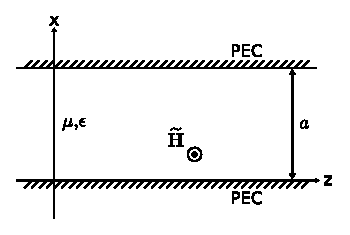
\includegraphics[width=0.8\columnwidth]{modules/m0177_fParallelPlateWaveguide.eps} 
% https://commons.wikimedia.org/wiki/File:TM_component_of_electric_field_in_parallel_plate_waveguide.svg
}}{For a z-x Cartesian coordinate system two parallel plates are a distance small a apart. The interior region is labeled small mu comma small epsilon. The magnetic field intensity is out of page.}
\end{center}
\centerline{\scriptsize 
\copyright~\hyperref[m0177_fParallelPlateWaveguide_Credit]{C.\ Wang} 
\href{https://creativecommons.org/licenses/by-sa/4.0/}{CC BY-SA 4.0} 
} % \centerline 
\caption{
\label{m0177_fParallelPlateWaveguide}
TM component of the electric field in a parallel plate waveguide.
}
\end{figure}
%
At the end of that section, we decomposed the problem into its TE and TM components.
In this section, we find the TM component of the fields in the waveguide.

``Transverse magnetic'' means the magnetic field vector is perpendicular to the plane of interest, and is therefore parallel to the conducting surfaces.
Thus, $\widetilde{\bf H} = \hat{\bf y}\widetilde{H}_y$, with no component in the $\hat{\bf x}$ or $\hat{\bf z}$ directions.
Following precisely the same reasoning employed in Section~\ref{m0173_Parallel_Plate_Waveguide_Introduction}, we find the governing equation for the magnetic component of TM field is:
%
\begin{equation}
\frac{\partial^2}{\partial x^2}\widetilde{H}_y + \frac{\partial^2}{\partial z^2}\widetilde{H}_y = - \beta^2 \widetilde{H}_y 
\label{m0177_eDH}
\end{equation}
%
The general solution to this partial differential equation is:
%
\begin{flalign}
\widetilde{H}_y =&~~~~~e^{-jk_z z} \left[ A e^{-jk_x x} + B e^{+jk_x x} \right] \nonumber \\
                 &+e^{+jk_z z} \left[ C e^{-jk_x x} + D e^{+jk_x x} \right] 
\label{m0177_eGS}
\end{flalign}
%
where 
$A$, $B$, $C$, and $D$ are complex-valued constants; and 
$k_x$ and $k_z$ are real-valued constants.
We have assigned variable names to these constants with advance knowledge of their physical interpretation; however, at this moment they remain simply unknown constants whose values must be determined by enforcement of boundary conditions.

Note that Equation~\ref{m0177_eGS} consists of two terms.
The first term includes the factor $e^{-jk_z z}$, indicating a wave propagating in the $+\hat{\bf z}$ direction, and
the second term includes the factor $e^{+jk_z z}$, indicating a wave propagating in the $-\hat{\bf z}$ direction.
If we impose the restriction that sources exist only on the left ($z<0$) side of Figure~\ref{m0177_fParallelPlateWaveguide}, and that there be no structure capable of wave scattering (in particular, reflection) on the right ($z>0$) side of Figure~\ref{m0177_fParallelPlateWaveguide}, then there can be no wave components propagating in the $-\hat{\bf z}$ direction.  In this case, $C=D=0$ and Equation~\ref{m0177_eGS} simplifies to:
%
\begin{equation}
\widetilde{H}_y = e^{-jk_z z} \left[ A e^{-jk_x x} + B e^{+jk_x x} \right] 
\label{m0177_eGS2}
\end{equation}

Before proceeding, let's make sure that Equation~\ref{m0177_eGS2} is actually a solution to Equation~\ref{m0177_eDH}.
As in the TE case, this check yields a constraint (in fact, the same constraint) on the as-yet undetermined parameters $k_x$ and $k_z$.
First, note:
%
\begin{equation}
\frac{\partial \widetilde{H}_y}{\partial x} = e^{-jk_z z} \left[-A e^{-jk_x x} + B e^{+jk_x x} \right]\left(jk_x\right) 
\label{m0177_edHydx}
\end{equation}
%
So:
%
\begin{flalign}
\frac{\partial^2 \widetilde{H}_y}{\partial x^2} &= e^{-jk_z z} \left[ A e^{-jk_x x} + B e^{+jk_x x} \right]\left(-k_x^2\right) \nonumber \\
                                                &= -k_x^2 \widetilde{H}_y
\end{flalign}
%
Next, note:
%
\begin{equation}
\frac{\partial \widetilde{H}_y}{\partial z}     = e^{-jk_z z} \left[ A e^{-jk_x x} + B e^{+jk_x x} \right]\left(-jk_z\right) 
\label{m0177_edHydz}
\end{equation}
%
So:
%
\begin{flalign}
\frac{\partial^2 \widetilde{H}_y}{\partial z^2} &= e^{-jk_z z} \left[ A e^{-jk_x x} + B e^{+jk_x x} \right]\left(-k_z^2\right) \nonumber \\
                                                &= -k_z^2 \widetilde{H}_y
\end{flalign}
%
Now summing these results:
%
\begin{equation}
\frac{\partial^2 \widetilde{H}_y}{\partial x^2} + \frac{\partial^2 \widetilde{H}_y}{\partial z^2} = -\left( k_x^2 + k_z^2 \right) \widetilde{H}_y
\label{m0177_eDE2}
\end{equation}
%
Comparing Equation~\ref{m0177_eDE2} to Equation~\ref{m0177_eDH}, we conclude that Equation~\ref{m0177_eGS2} is a solution to Equation~\ref{m0177_eDH} under the constraint that:
%
\begin{equation}
\beta^2 = k_x^2 + k_z^2
\label{m0177_eBeta}
\end{equation}
%
This is precisely the same constraint identified in the TE case, and confirms that $k_x$ and $k_y$ are in fact the components of the propagation vector
%
\begin{equation}
{\bf k} \triangleq \beta\hat{\bf k} = \hat{\bf x}k_x + \hat{\bf y}k_y + \hat{\bf z}k_z
\end{equation}
%
where $\hat{\bf k}$ is the unit vector pointing in the direction of propagation, and $k_y=0$ in this particular problem. 

Our objective in this section is to determine the \emph{electric} field component of the TM field.  
The electric field may be obtained from the magnetic field using Ampere's law:
\index{Ampere's law!general form}
%
\begin{equation}
\nabla \times \widetilde{\bf H} = j\omega\epsilon \widetilde{\bf E}
\end{equation}
%
Thus:
%
\begin{flalign}
\widetilde{\bf E} &= \frac{1}{j\omega\epsilon}~\nabla \times \widetilde{\bf H} \nonumber \\
                  &= \frac{1}{j\omega\epsilon}~\nabla \times \left(\hat{\bf y}\widetilde{H}_y\right) 
\end{flalign}
%
The relevant form of the curl operator is Equation~\ref{m0139_eCurlCart} (Appendix~\ref{m0139_Vector_Operators}).
Although the complete expression consists of 6 terms, all but 2 of these terms are zero because the $\hat{\bf x}$ and $\hat{\bf z}$ components of $\widetilde{\bf H}$ are zero.
The two remaining terms are 
$-\hat{\bf x}\partial \widetilde{H}_y/\partial z$ and
$+\hat{\bf z}\partial \widetilde{H}_y/\partial x$.
Thus:
%
\begin{equation}
\widetilde{\bf E} = \frac{1}{j\omega\epsilon}~\left( -\hat{\bf x}\frac{\partial\widetilde{H}_y}{\partial z} +\hat{\bf z}\frac{\partial\widetilde{H}_y}{\partial x} \right) 
\label{m0177_eE}
\end{equation}
%
We may further develop this expression using Equations~\ref{m0177_edHydx} and \ref{m0177_edHydz}.
We find the $\hat{\bf x}$ component of $\widetilde{\bf E}$ is:
%
\begin{equation}
\widetilde{E}_x = \frac{k_z}{\omega\epsilon}~e^{-jk_z z} \left[ A e^{-jk_x x} + B e^{+jk_x x} \right]
\label{m0177_eEx}
\end{equation}
%
and the $\hat{\bf z}$ component of $\widetilde{\bf E}$ is:
%
\begin{equation}
\widetilde{E}_z = \frac{k_x}{\omega\epsilon}~e^{-jk_z z} \left[ -A e^{-jk_x x} + B e^{+jk_x x} \right]
\label{m0177_eEz}
\end{equation}

The solution has now been reduced to the problem of finding the constants $A$, $B$, and either $k_x$ or $k_z$.
This is accomplished by enforcing the relevant boundary conditions.
In general, the component of the electric field which is tangent to a perfectly-conducting surface is zero.
Applied to the present (TM) case, this means 
$\widetilde{E}_z\left(x=0\right) = 0$ and
$\widetilde{E}_z\left(x=a\right) = 0$.
Referring to Equation~\ref{m0177_eEz}, the boundary condition at $x=0$ means
%
\begin{equation}
\frac{k_x}{\omega\epsilon}~e^{-jk_z z} \left[ -A \left(1\right) + B \left(1\right) \right] = 0
\end{equation} 
%
The factor $e^{-jk_z z}$ always has unit magnitude, and so cannot be zero. 
We could require $k_x$ to be zero, but this is unnecessarily restrictive.
Instead, we require $A=B$ and we may rewrite Equation~\ref{m0177_eEz} as follows:
%
\begin{equation}
\widetilde{E}_z = \frac{B k_x}{\omega\epsilon}~e^{-jk_z z} \left[ e^{+jk_x x} - e^{-jk_x x} \right] 
\end{equation}
%
This expression is simplified using a trigonometric identity:
%
\begin{equation}
\sin{k_x a} = \frac{1}{2j}\left[ e^{+jk_x a} - e^{-jk_x a} \right]
\end{equation} 
%
Thus:
%
\begin{equation}
\widetilde{E}_z = \frac{j2B k_x}{\omega\epsilon} e^{-jk_z z} \sin k_x x
\end{equation}
%
Now following up with $\widetilde{E}_x$, beginning from Equation~\ref{m0177_eEx}:
%
\begin{flalign}
\widetilde{E}_x &= \frac{k_z}{\omega\epsilon}~e^{-jk_z z} \left[ A e^{-jk_x x} + B e^{+jk_x x} \right] \nonumber \\
                &= \frac{B k_z}{\omega\epsilon}~e^{-jk_z z} \left[ e^{-jk_x x} + e^{+jk_x x} \right] \nonumber \\
                &= \frac{2B k_z}{\omega\epsilon}~e^{-jk_z z} \cos k_x x
\end{flalign}
%
For convenience we define the following complex-valued constant:
%
\begin{equation}
E_{x0}\triangleq \frac{2B k_z}{\omega\epsilon}
\end{equation}
% 
This yields the following simpler expression:
%
\begin{equation}
\widetilde{E}_x = E_{x0}~e^{-jk_z z} \cos k_x x 
\end{equation}
%
Now let us apply the boundary condition at $x=a$ to $\widetilde{E}_{z}$:
%
\begin{equation}
\frac{j2B k_z}{\omega\epsilon} e^{-jk_z z} \sin k_x a  = 0
\end{equation} 
%
Requiring $B=0$ or $k_z=0$ yields only trivial solutions, therefore, it must be true that 
%
\begin{equation}
\sin{k_x a} = 0
\end{equation} 
%
This in turn requires that
%
\begin{equation}
k_x a = m \pi 
\end{equation}
%
where $m$ is an integer.
Note that this is precisely the same relationship that we identified in the TE case.
There is an important difference, however.
In the TE case, $m=0$ was not of interest because this yields $k_x=0$, and the associated field turned out to be identically zero.
In the present (TM) case, $m=0$ also yields $k_x=0$, but the associated field is not necessarily zero.
That is, for $m=0$, $\widetilde{E}_z=0$ but $\widetilde{E}_x$ is not necessarily zero.  
Therefore, $m=0$ as well as $m=1$, $m=2$, and so on are of interest in the TM case.

At this point, we have uncovered a family of solutions with $m=0,1,2,...$.
Each solution is referred to as a \emph{mode}, and is associated with a particular value of $k_x$.
\index{mode}
In the discussion that follows, we shall find that the consequences are identical to those identified in the TE case, except that $m=0$ is now also allowed.
Continuing:
The value of $k_z$ for mode~$m$ is obtained using Equation~\ref{m0177_eBeta} as follows:
%
\begin{flalign}
k_z &= \sqrt{\beta^2-k_x^2} \nonumber \\
    & =\sqrt{\beta^2-\left(\frac{m\pi}{a}\right)^2}
\end{flalign}
%
Since $k_z$ is specified to be real-valued, we require:
%
\begin{equation}
\beta^2-\left(\frac{m\pi}{a}\right)^2 > 0
\end{equation}
%
This constrains $\beta$; specifically:
%
\begin{equation}
\beta > \frac{m\pi}{a}
\end{equation}
%
Recall that $\beta=\omega\sqrt{\mu\epsilon}$ and $\omega=2\pi f$ where $f$ is frequency.
Solving for $f$, we find:
%
\begin{equation}
f > \frac{m}{2a\sqrt{\mu\epsilon}}
\end{equation}
%
Thus, each mode exists only above a certain frequency, which is different for each mode. 
This \emph{cutoff frequency}
\index{cutoff frequency}
$f_c$ for mode $m$ is given by 
 %
\begin{equation}
\boxed{
f_c^{(m)} \triangleq \frac{m}{2a\sqrt{\mu\epsilon}}
}
\label{m0177_efcm}
\end{equation}
%
At frequencies below the cutoff frequency for mode $m$, modes $0$ through $m-1$ exhibit imaginary-valued $k_z$ and therefore do no propagate.
Also, note that the cutoff frequency for $m=0$ is zero, and so this mode is always able to propagate.
That is, the $m=0$ mode may exist for any $a>0$ and any $f>0$.
Once again, this is a remarkable difference from the TE case, for which $m=0$ is not available.

Let us now summarize the solution.
With respect to Figure~\ref{m0177_fParallelPlateWaveguide}, we find that the electric field component of the TM field is given by:
%
\begin{equation}
\boxed{
\widetilde{\bf E} = \sum_{m=0}^{\infty} \left[ \hat{\bf x} \widetilde{E}_x^{(m)} + \hat{\bf z} \widetilde{E}_z^{(m)} \right]
}
\label{m0177_eEsum}
\end{equation}
%
where
%
\begin{equation}
\boxed{
\widetilde{E}_x^{(m)} \triangleq \begin{cases}
                                   0,                             & f<f_c^{(m)} \\
                                   E_{x0}^{(m)} e^{-jk_z^{(m)} z} \cos k_x^{(m)} x, & f\ge f_c^{(m)} 
                                 \end{cases}
}
\end{equation}
%
and
%
\begin{equation}
\boxed{
\widetilde{E}_z^{(m)} \triangleq \begin{cases}
                                   0,                             & f<f_c^{(m)} \\
                                   j\frac{k_x^{(m)}}{k_z^{(m)}}E_{x0}^{(m)} e^{-jk_z^{(m)} z} \sin k_x^{(m)} x, & f\ge f_c^{(m)} 
                                 \end{cases}
}
\end{equation}
%
where $m$ enumerates modes ($m=0,1,2,...$) and
%
\begin{equation}
\boxed{
k_z^{(m)} \triangleq \sqrt{\beta^2-\left[k_x^{(m)}\right]^2} 
}
\end{equation}
%
\begin{equation}
\boxed{
k_x^{(m)} \triangleq m\pi/a 
}
\label{m0177_ekxma}
\end{equation}
%
Finally, the coefficients $E_{x0}^{(m)}$ depend on sources and/or boundary conditions to the left of the region of interest.

%%%%%%%%%%%%%%%%%%%%%%%%%%%%%%%%%%%%%%%%%%%%%%%
%ORB HIGHLIGHT
\begin{mdframed}[backgroundcolor=yellow!20,nobreak=true] 
For the scenario depicted in Figure~\ref{m0177_fParallelPlateWaveguide}, the electric field component of the TM solution is given by Equation~\ref{m0177_eEsum} with modal components determined as indicated by Equations~\ref{m0177_efcm}--\ref{m0177_ekxma}.  This solution presumes all sources lie to the left of the region of interest, with no additional sources or boundary conditions to the right of the region of interest.
\end{mdframed}
%%%%%%%%%%%%%%%%%%%%%%%%%%%%%%%%%%%%%%%%%%%%%%%
  
The $m=0$ mode, commonly referred to as the ``TM$_0$'' mode, is of particular importance in the analysis of microstrip transmission line, and is addressed in Section~\ref{m0220_Parallel_Plate_Waveguide_TM0_Mode}.

\index{waveguide!parallel plate|)}


